\documentclass[tikz, border=10pt]{standalone}
\usepackage{tikz}
\usetikzlibrary{shapes.geometric, arrows.meta, positioning, fit, calc, backgrounds, shadows, shapes.arrows, shapes.misc}
\usepackage{amsmath, amssymb}

% Colors
\definecolor{lightcyan}{RGB}{220, 245, 255}
\definecolor{myblue}{RGB}{200, 220, 255}
\definecolor{mygreen}{RGB}{210, 255, 180}
\definecolor{darkgreen}{RGB}{100, 180, 80}
\definecolor{myorange}{RGB}{255, 210, 150}
\definecolor{mypink}{RGB}{255, 180, 190}
\definecolor{mydarkpink}{RGB}{230, 100, 120}
\definecolor{myviolet}{RGB}{200, 160, 255}
\definecolor{arrowblack}{RGB}{0, 0, 0}

\begin{document}
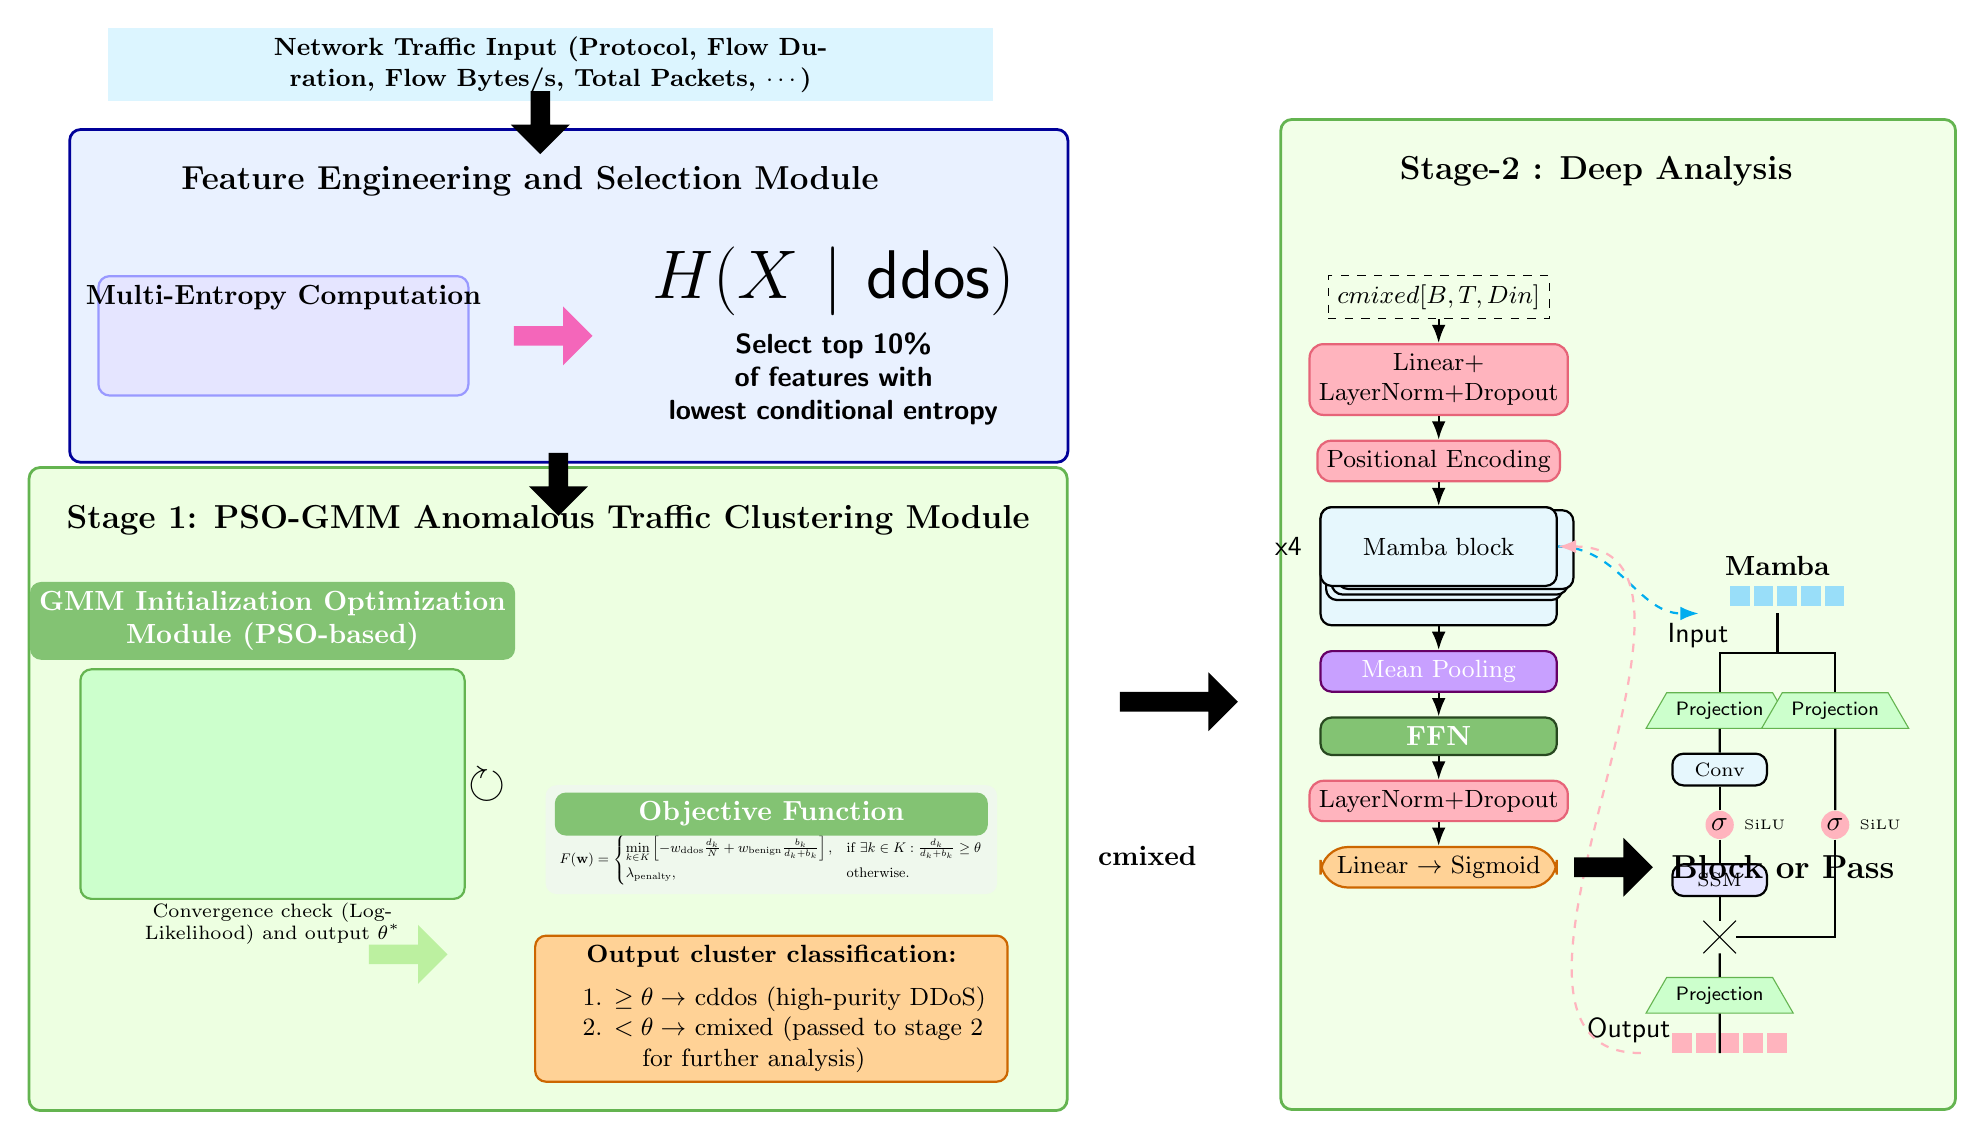
\begin{tikzpicture}[
    font=\sffamily,
    >=Latex,
    node distance=0.5cm,
    % Styles
    basebox/.style={draw, rounded corners, align=center, line width=0.8pt, font=\small},
    titlebox/.style={fill=lightcyan, draw=none, minimum height=0.8cm, text width=11cm, align=center, font=\bfseries\small},
    sectiontitle/.style={font=\bfseries\large, align=center},
    container/.style={draw, line width=1pt, rounded corners, inner sep=10pt},
    process/.style={basebox, fill=white, draw=black, minimum height=0.7cm},
    darkgreenbox/.style={basebox, fill=darkgreen!80, draw=darkgreen!40!black, text=white, font=\bfseries},
    orangebox/.style={basebox, fill=myorange, draw=orange!80!black},
    pinkbox/.style={basebox, fill=mypink, draw=mydarkpink, rounded corners=5pt},
    violetbox/.style={basebox, fill=myviolet, draw=violet!80!black, text=white},
    ]

    % =========================================================
    % 1. TOP: Input
    % =========================================================
    \node[titlebox] (input) {Network Traffic Input (Protocol, Flow Duration, Flow Bytes/s, Total Packets, $\cdots$)};
    
    \node[single arrow, fill=black, rotate=-90, minimum height=0.8cm, below=0.2cm of input] (arrow1) {};

    % =========================================================
    % 2. Feature Engineering
    % =========================================================
    % Define Content First
    \node[sectiontitle, below=0.5cm of arrow1] (fe_title) {Feature Engineering and Selection Module};
    
    % Group: Entropy
    \node[below=1.5cm of fe_title, xshift=-3cm] (renyi) [process, minimum width=1.2cm] {Rényi};
    \node[process, minimum width=1.2cm, left=0.2cm of renyi] (shannon) {Shannon};
    \node[process, minimum width=1.2cm, right=0.2cm of renyi] (min) {Min};
    
    % Wrapper for Entropy
    \node[basebox, fill=blue!10, draw=blue!40, fit={(shannon) (min) ($(renyi)+(0,0.8)$)}, inner sep=5pt] (entropy_box) {};
    \node[anchor=north, font=\bfseries] at (entropy_box.north) {Multi-Entropy Computation};
    
    % Formula
    \node[right=2cm of entropy_box, align=center, text width=5cm] (formula) {
        {\Huge $H(X \mid \text{ddos})$} \\[0.5em]
        \textbf{Select top 10\% of features with \\ lowest conditional entropy}
    };
    
    % Arrow between them
    \node[single arrow, fill=magenta!60, minimum height=1cm] at ($(entropy_box.east)!0.5!(formula.west)$) {};

    % Container (Background)
    \begin{scope}[on background layer]
        \node[container, fill=myblue!40, draw=blue!60!black, fit={(fe_title) (entropy_box) (formula)}, inner sep=10pt] (fe_container) {};
    \end{scope}

    % =========================================================
    % 3. Stage 1
    % =========================================================
    \node[single arrow, fill=black, rotate=-90, minimum height=0.8cm, below=0.2cm of fe_container] (arrow2) {};
    \node[sectiontitle, below=0.2cm of arrow2] (st1_title) {Stage 1: PSO-GMM Anomalous Traffic Clustering Module};
    
    % GMM Logic (Left)
    % EM Box
    \node[basebox, fill=darkgreen!10, draw=black, minimum width=4.5cm, minimum height=2.5cm, below=1.8cm of st1_title, xshift=-3.5cm] (em_box) {};
    
    \node[below=0.1cm of em_box.north, font=\bfseries] {EM algorithm iteration};
    \node[process, fill=green!5, minimum width=4cm, below=0.5cm of em_box.north] (estep) {E-Step $\mid \to \mathbf{\gamma}$};
    \node[process, fill=green!5, minimum width=4cm, below=0.2cm of estep] (mstep) {M-Step $\mid \to \{ \mathbf{\mu}, \mathbf{\Sigma}, \mathbf{\pi} \}$};
    
    % Cycle and text
    \node[right=0.1cm of em_box, font=\LARGE] {$\boldsymbol{\circlearrowright}$};
    \node[below=0.1cm of em_box, align=center, font=\scriptsize] {Convergence check (Log-\\Likelihood) and output $\theta^*$};
    
    % Wrapper GMM
    \node[basebox, fill=green!20, draw=darkgreen, fit={(em_box) ($(em_box)+(0,1.3)$) ($(em_box)+(0,-0.8)$)}, inner sep=5pt] (gmm_logic) {};
    \node[above=0.1cm of em_box, font=\bfseries, align=center, fill=darkgreen!80, text=white, minimum width=4.8cm, rounded corners] at (gmm_logic.north) {GMM Initialization Optimization \\ Module (PSO-based)};

    % Objective Function (Right Top)
    \node[basebox, fill=darkgreen!10, draw=none, right=1cm of gmm_logic, anchor=north west] (obj_box) {
         \\[1.5em]
        \resizebox{5.5cm}{!}{
        $F(\mathbf{w}) =
        \begin{cases}
        \min\limits_{k \in K} \left[ -w_{\text{ddos}} \frac{d_k}{N} + w_{\text{benign}} \frac{b_k}{d_k + b_k} \right], & \text{if } \exists k \in K : \frac{d_k}{d_k + b_k} \ge \theta \\
        \lambda_{\text{penalty}}, & \text{otherwise}.
        \end{cases}$
        }
    };
    \node[below=0.1cm of obj_box.north, font=\bfseries, align=center, fill=darkgreen!80, text=white, minimum width=5.5cm, rounded corners] at (obj_box.north) {Objective Function};

    % Output Classification (Right Bottom)
    \node[basebox, fill=myorange, draw=orange!80!black, below=0.5cm of obj_box, minimum width=6cm, align=left] (class_box) {
        \textbf{\hspace{1em}Output cluster classification:} \\[0.5em]
        \hspace{1em}1. $\ge \theta \to$ cddos (high-purity DDoS) \\
        \hspace{1em}2. $< \theta \to$ cmixed (passed to stage 2 \\ \hspace{3em} for further analysis)
    };

    % Arrow inside Stage 1
    \node[single arrow, fill=mygreen!80!darkgreen, minimum height=1cm] at ($(gmm_logic.south)!0.5!(class_box.west)$) {};

    % Container (Background)
    \begin{scope}[on background layer]
        \node[container, fill=mygreen!40, draw=darkgreen, fit={(st1_title) (gmm_logic) (class_box) (obj_box)}, inner sep=10pt] (st1_container) {};
    \end{scope}

    % =========================================================
    % 4. Stage 2 (Right Column)
    % =========================================================
    % Stack
    \node[pinkbox, minimum width=3cm, right=4cm of input, yshift=-4cm] (lin1) {Linear+\\LayerNorm+Dropout};
    \node[above=0.3cm of lin1, font=\small, draw, dashed] (input_dim) {$cmixed[B, T, Din]$};
    \draw[->, thick] (input_dim) -- (lin1);
    
    \node[pinkbox, minimum width=3cm, below=0.3cm of lin1] (posenc) {Positional Encoding};
    
    % Mamba Stack
    \node[basebox, fill=cyan!10, draw=black, minimum width=3cm, minimum height=1.5cm, below=0.3cm of posenc] (mamba_stack) {};
    \foreach \i in {1,2,3} { \node[basebox, fill=cyan!10, draw=black, minimum width=3cm, minimum height=1cm] at ($(mamba_stack.center) + (\i*2pt, \i*2pt)$) {}; }
    \node[basebox, fill=cyan!10, draw=black, minimum width=3cm, minimum height=1cm, below=0.3cm of posenc] (mamba_block) {Mamba block};
    \node[left=0.1cm of mamba_block] {x4};
    
    \node[violetbox, minimum width=3cm, below=0.3cm of mamba_stack] (pool) {Mean Pooling};
    \node[darkgreenbox, minimum width=3cm, below=0.3cm of pool] (ffn) {FFN};
    \node[pinkbox, minimum width=3cm, below=0.3cm of ffn] (lin2) {LayerNorm+Dropout};
    \node[orangebox, rounded corners=10pt, minimum width=3cm, below=0.3cm of lin2] (sigmoid) {Linear $\to$ Sigmoid};

    % Stack Arrows
    \draw[->, thick] (lin1) -- (posenc);
    \draw[->, thick] (posenc) -- (mamba_block);
    \draw[->, thick] (mamba_stack) -- (pool);
    \draw[->, thick] (pool) -- (ffn);
    \draw[->, thick] (ffn) -- (lin2);
    \draw[->, thick] (lin2) -- (sigmoid);
    
    % Detail View
    \node[right=2cm of mamba_stack, font=\bfseries] (detail_title) {Mamba};
    \coordinate (detail_top) at ($(detail_title)+(0,-0.5)$);
    
    % Input Array
    \foreach \x in {-2,-1,0,1,2} \fill[cyan!40] ($(detail_top) + (\x*0.3, 0)$) rectangle ++(0.25, 0.25);
    \coordinate (d_in) at ($(detail_top) + (0, -0.1)$);
    \node[below left=0cm and 0.5cm of d_in] {Input};
    
    % Split
    \coordinate (split) at ($(d_in) + (0, -0.5)$);
    \draw[thick] (d_in) -- (split);
    
    % Branches
    \node[trapezium, draw=darkgreen, fill=green!20, trapezium left angle=60, trapezium right angle=60, minimum width=1.2cm, below left=0.5cm and 0.5cm of split] (proj1) {\scriptsize Projection};
    \node[basebox, fill=cyan!10, below=0.3cm of proj1, minimum width=1.2cm] (conv) {\scriptsize Conv};
    \node[circle, fill=mypink, inner sep=1pt, below=0.3cm of conv] (silu1) {$\sigma$}; \node[right=0cm of silu1, font=\tiny] {SiLU};
    \node[basebox, fill=blue!10, below=0.3cm of silu1, minimum width=1.2cm] (ssm) {\scriptsize SSM};
    
    \node[trapezium, draw=darkgreen, fill=green!20, trapezium left angle=60, trapezium right angle=60, minimum width=1.2cm, below right=0.5cm and 0.5cm of split] (proj2) {\scriptsize Projection};
    \node[circle, fill=mypink, inner sep=1pt] (silu2) at (silu1 -| proj2) {$\sigma$}; \node[right=0cm of silu2, font=\tiny] {SiLU};
    
    % Connections
    \draw[thick] (split) -| (proj1);
    \draw[thick] (split) -| (proj2);
    \draw[thick] (proj1) -- (conv);
    \draw[thick] (conv) -- (silu1);
    \draw[thick] (silu1) -- (ssm);
    \draw[thick] (proj2) -- (silu2);
    
    % Multiply
    \node[circle, draw, cross out, inner sep=2pt, minimum size=0.4cm, below=0.3cm of ssm] (mult) {};
    \draw[thick] (ssm) -- (mult);
    \draw[thick] (silu2) |- (mult);
    
    % Final Proj
    \node[trapezium, draw=darkgreen, fill=green!20, trapezium left angle=60, trapezium right angle=60, minimum width=1.2cm, below=0.3cm of mult] (proj_final) {\scriptsize Projection};
    \draw[thick] (mult) -- (proj_final);
    
    % Output Array
    \coordinate (d_out) at ($(proj_final.south) + (0, -0.5)$);
    \foreach \x in {-2,-1,0,1,2} \fill[mypink] ($(d_out) + (\x*0.3, 0)$) rectangle ++(0.25, 0.25);
    \node[above left=0cm and 0.5cm of d_out] {Output};
    \draw[thick] (proj_final) -- (d_out);
    
    % Detail Box (Back)
    \begin{scope}[on background layer]
        \node[process, fit={(detail_title) (d_out) (proj1) (proj2)}, inner sep=10pt] (detail_whitebox) {};
    \end{scope}

    % Zoom Lines
    \draw[dashed, thick, cyan, ->] (mamba_block.east) to[out=0, in=180] ($(d_in)+(-1,0)$);
    \draw[dashed, thick, mypink, ->] ($(d_out)+(-1,0)$) to[out=180, in=0] (mamba_block.east);

    % Stage 2 Container
    \node[sectiontitle, above=1cm of input_dim, xshift=2cm] (st2_title) {Stage-2 : Deep Analysis};
    \begin{scope}[on background layer]
        \node[container, fill=mygreen!30, draw=darkgreen, fit={(st2_title) (lin1) (sigmoid) (detail_whitebox)}, inner sep=10pt] (st2_container) {};
    \end{scope}

    % Link from Stage 1 to Stage 2
    \node[single arrow, fill=black, minimum height=1.5cm] at ($(st1_container.east)!0.5!(st2_container.west)$) {};
    \node[above=3cm of st1_container.south east, xshift=1cm, font=\bfseries] {cmixed};

    % Final Output
    \node[single arrow, fill=black, minimum height=1cm, right=0.2cm of sigmoid] (final_arrow) {};
    \node[right=0.1cm of final_arrow, font=\bfseries\large] {Block or Pass};

\end{tikzpicture}
\end{document}
